\documentclass{standalone}
\usepackage{tikz}
\usetikzlibrary{calc}

\begin{document}
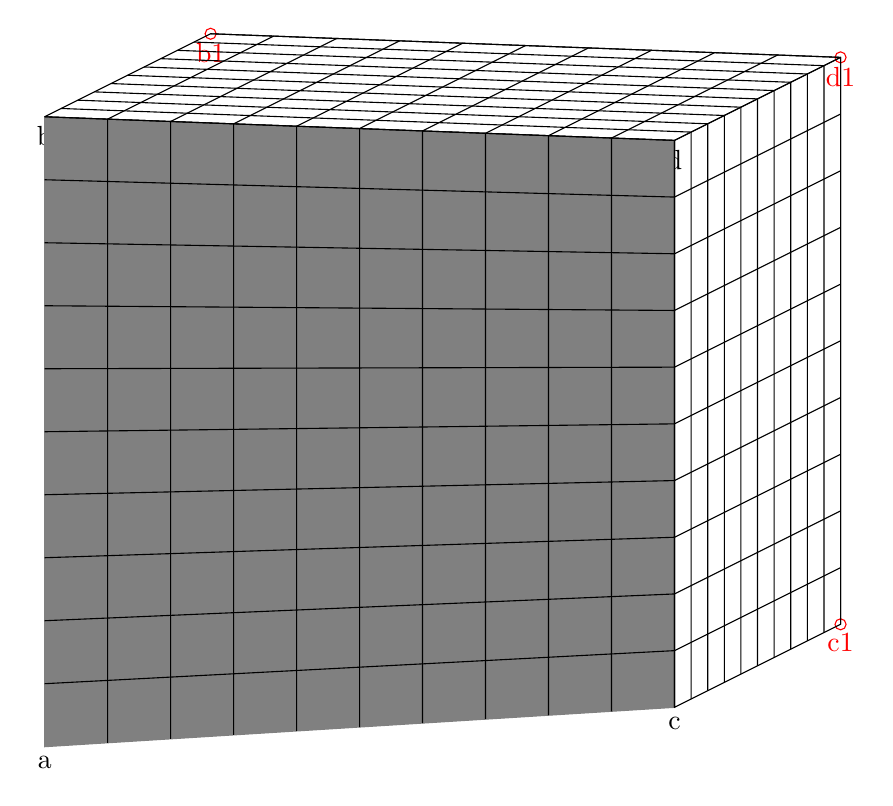
\begin{tikzpicture}

   \coordinate (Center) at (0,0);
   \coordinate (a) at (-4,-4);
   \coordinate (b) at (-4,4);
   \coordinate (c) at (4,-3.5);
   \coordinate (d) at (4,3.7);

   \coordinate[yshift=30,xshift=60] (a1) at (a);
   \coordinate[yshift=30,xshift=60] (b1) at (b);
   \coordinate[yshift=30,xshift=60] (c1) at (c);
   \coordinate[yshift=30,xshift=60] (d1) at (d);

\draw[color=red] (a1) circle (2pt) node[below] {a1};
\draw[color=red] (b1) circle (2pt) node[below] {b1};
\draw[color=red] (c1) circle (2pt) node[below] {c1};
\draw[color=red] (d1) circle (2pt) node[below] {d1};


   \node[below] at (a) {a};
   \node[below] at (b) {b};
   \node[below] at (c) {c};
   \node[below] at (d) {d};

   %\draw[step=1cm,gray!30,very thin] (-6.5,-6.5) grid (6.5,6.5);
   \draw (Center) circle (2pt);
    
   \draw[fill,color=gray] (a) -- (b) -- (d) -- (c) -- cycle;
   \draw (b) -- (b1) -- (d1) -- (c1) -- (c) -- (d) -- (b);

\foreach \x in {0.1,0.2,0.3,...,1.1}
   \draw ($(a)!\x!(c)$) -- ($(b)!\x!(d)$) -- ($(b1)!\x!(d1)$);
\foreach \x in {0.1,0.2,0.3,...,1.1}
   \draw ($(a)!\x!(b)$) -- ($(c)!\x!(d)$) -- ($(c1)!\x!(d1)$); 
\foreach \x in {0.1,0.2,0.3,...,1.1}
   \draw ($(b)!\x!(b1)$) -- ($(d)!\x!(d1)$) -- ($(c)!\x!(c1)$);   
   

   %\draw ($(a)$) circle (2pt);

\end{tikzpicture}

\end{document}